\section{Neural Networks}
\subsection{Why Neural Networks?}
Neural networks are needed to resolve the limitations of other seen models. More in depth:
\begin{itemize}
    \item \textbf{Perceptron:} can only learn linearly separable functions;
    \item \textbf{Kernel Machines:} add the concept of non-linearity, but the choice of the appropriate kernel is not trivial;
\end{itemize}
\subsection{Multi Layer Perceptron}
A Multi Layer Perceptron (MLP) is a network of interconnected neurons, organized in layers. Neuorns from one layer
sends their output to the neurons of the next layer. The first layer is called \textit{input layer}, one or mode \textit{hidden layers}
are in the middle, and the last layer is called \textit{output layer}.

\begin{tikzpicture}[
    node distance=12mm,
    every node/.style={draw,circle,minimum size=8mm},
    input/.style={fill=purple!50},
    hidden/.style={fill=green!20},
    output/.style={fill=red!50},
    arrow/.style={-{Latex[length=2mm]},thin}
]

% INPUT LAYER
\node[input] (i1) at (0,0)  {};
\node[input] (i2) at (1.2,0) {};
\node[input] (i3) at (2.4,0) {};
\node[input] (i4) at (3.6,0) {};
\node[input] (i5) at (4.8,0) {};
\node[draw=none] at (2.4,-1) {$x$};
\node[draw=none] at (-1.3,0) {Input layer};

% LAYER 1 (3 nodes)
\node[hidden] (h11) at (1.0,1.5)  {};
\node[hidden] (h12) at (2.4,1.5)  {};
\node[hidden] (h13) at (3.8,1.5)  {};
\node[draw=none] at (-1.3,1.5) {Layer 1};

% LAYER 2 (3 nodes)
\node[hidden] (h21) at (1.0,3.0)  {};
\node[hidden] (h22) at (2.4,3.0)  {};
\node[hidden] (h23) at (3.8,3.0)  {};
\node[draw=none] at (-1.3,3.0) {Layer 2};

% LAYER 3 (unchanged)
\node[hidden] (h31) at (1.2,4.5)  {};
\node[hidden] (h32) at (2.4,4.5)  {};
\node[hidden] (h33) at (3.6,4.5)  {};
\node[draw=none] at (-1.3,4.5) {Layer 3};

% OUTPUT LAYER
\node[output] (o1) at (2.4,6.0) {};
\node[draw=none] at (-1.3,6.0) {Output layer};

% Connections
\foreach \i in {1,...,5}{
   \foreach \h in {11,12,13}{
     \draw[arrow] (i\i) -- (h\h);
   }
}
\foreach \a in {11,12,13}{
   \foreach \b in {21,22,23}{
     \draw[arrow] (h\a) -- (h\b);
   }
}
\foreach \a in {21,22,23}{
   \foreach \b in {31,32,33}{
     \draw[arrow] (h\a) -- (h\b);
   }
}
\foreach \a in {31,32,33}{
     \draw[arrow] (h\a) -- (o1);
}

% Equations on the right
\node[draw=none,anchor=west,text width=7cm] at (6,4.5)
  {$\phi_3(x)=\sigma(W_3\phi_2(x))=\sigma(W_3\sigma(W_2\sigma(W_1 x)))$};
\node[draw=none,anchor=west,text width=7cm] at (6,3.0)
  {$\phi_2(x)=\sigma(W_2\phi_1(x))=\sigma(W_2\sigma(W_1 x))$};
\node[draw=none,anchor=west,text width=7cm] at (6,1.5)
  {$\phi_1(x)=\sigma(W_1 x)$};
\node[draw=none,anchor=west,text width=7cm] at (6,6.0)
  {$f(x)=w^\top \phi_3(x)$};
\end{tikzpicture}

Where:
\begin{itemize}
    \item $\boldsymbol{x}$ is the input vector;
    \item $\phi_i(x)$ is the output of layer $i$, learned from the data during training.
    \[\phi_i(x) = \sigma(W_i \boldsymbol{x})\]
    \item $W_i$ is the weight matrix of layer $i$. It's dimensions depend on the number of neurons in layer $i$. 
    Each row contains the weights associated to a neuron. Computing $W_i \boldsymbol{x}$ will return a vector
    which contains the weighted sum of the inputs for each neuron in layer $i$.
    \item $\sigma(\cdot)$ is a non-linear activation function, applied element-wise.
\end{itemize}
The final output is computed as a linear combination in the new feature space created by the hidden layers.
Differently from SVMs, where the kernel is chosen \textit{a priori}, in MLPs the transformation is learned from data. The only
downside is that training is requires more data and more computational power.
\subsubsection{Activation Functions}
Activation functions introduce non-linearity in the model. We will analyze some proposed functions:

\paragraph{Threshold activation:}
the treshold activation, already seen in the perceptron model, is defined as:
\[ f(\boldsymbol{x}) = sign(\boldsymbol{w}^T \boldsymbol{x}) \]
It's cannot be used in MLPs, since it's derivative is zero almost everywhere, apart from the discontinuity in zero (not differentiable). 
This makes impossible to use gradient-based optimization methods for training.

\paragraph{Sigmoid activation:}
The sigmoid activation function is defined as:
\[ f(\boldsymbol{x} = \sigma(\boldsymbol{w}^T \boldsymbol{x}) = \frac{1}{1 + e^{-\boldsymbol{w}^T \boldsymbol{x}}} \]
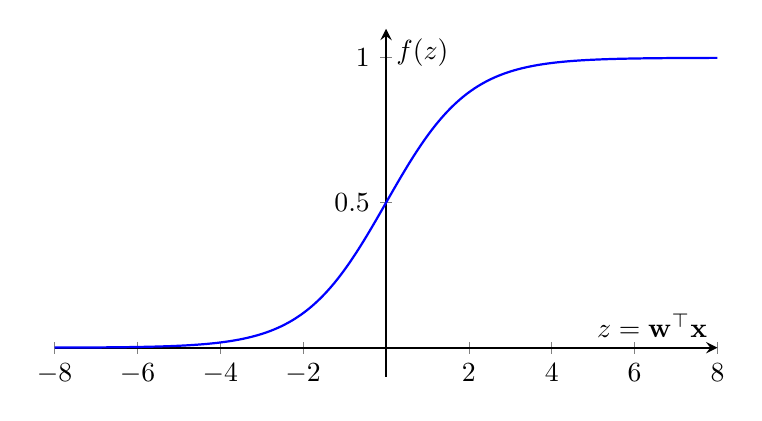
\begin{tikzpicture}
\begin{axis}[
    axis lines = middle,
    xlabel = {$z = \mathbf{w}^\top \mathbf{x}$},
    ylabel = {$f(z)$},
    ymin = -0.1, ymax = 1.1,
    samples = 200,
    domain = -8:8,
    width=10cm,
    height=6cm,
    thick,
]

\addplot[blue] {1/(1 + exp(-x))};
\end{axis}
\end{tikzpicture}
It represents a smooth approximation of the threshold function. It is approximately linear around zero, which helps in gradient-based optimization.
However, for large positive or negative values of $z$, the function saturates (approaches 0 or 1), causing the gradient to vanish.
\subsubsection{Output Layer}
The output layer of a neural network produces the final predictions. The function used can be 
different from the one used in hidden layers and heavily depends on the task at hand.
\\We will now analyze the activation functions used in the output layer for different tasks.
\paragraph{Binary Classification:} for binary classification tasks, only one output neuron $o(\boldsymbol{x})$ is needed.
The output activation function is usually the sigmoid activation function, which maps the output to the range (0, 1). It is defined as:
\[ f(\boldsymbol{x}) = \sigma(o(\boldsymbol{x})) = \frac{1}{1 + e^{-o(\boldsymbol{x})}} \]
This output can be interpreted as the probability of belonging to the positive class.
To obtain the final class label, a threshold (usually 0.5) is applied:
\[ y^* = sign(f(\boldsymbol{x}) - 0.5) \]

\paragraph{Multi-class Classification:} for multi-class classification, similar to what was done with single layer perceptrons, a one vs all approach can be used.
This requires $K$ output neurons, one for each class. The softmax activation function is commonly used in this case, defined as:
\[ f_i(\boldsymbol{x}) = \frac{e^{o_i(\boldsymbol{x})}}{\sum_{j=1}^{K} e^{o_j(\boldsymbol{x})}} \quad \text{for } i = 1, 2, \ldots, K \]
This function converts the raw output scores into probabilities that sum to 1 across all classes. This is not activated element-wise, but
it is a layer-wise activation function.
The predicted class is the one with the highest probability:
\[ y^* = \arg\max_{i} f_i(\boldsymbol{x}) \] 

\paragraph{Regression:} for regression tasks, where the output is a continuous value, the decision is the value of the output neuron itself.

\subsubsection{representational power of MLPs}
In this section we will analyze the representational power of MLPs on different tasks.
\begin{itemize}
    \item \textbf{Boolean functions:} any boolean function can be represented by a MLP with two layers of units. This can be done using CNF or DNF, but it would require
    an exponential number of hidden units in the worst case;
    \item \textbf{Continuous functions:} any bounded continuous function can be approximated arbitrarily well by a MLP with two layers of units (using sigmoid activations).
    \item \textbf{Arbitrary functions:} any function can be approximated arbitrarily well by a MLP with three layers of units (using sigmoid activations).
\end{itemize}

\subsection{Training Multi Layer Perceptrons}
Similarly to other models, MLPs are trained by minimizing a loss function on the training data. Different loss functions can be used depending on the task at hand.
\subsubsection{Loss Functions}
\paragraph{Binary Classification:}
For binary classification tasks, the binary cross-entropy loss is commonly used. It is defined as:
\[ L(y, f(\boldsymbol{x})) = - (y \log(f(\boldsymbol{x})) + (1 - y) \log(1 - f(\boldsymbol{x}))) \]
This can be interpreted as a switch function between two log-likelihoods, depending on the true label $y$. By putting the minus sign,
we convert the maximization problem into a minimization one (from a likelihood to a loss).

\paragraph{Multi-class Classification:}
For multi-class classification tasks, the cross-entropy loss is used. It is defined as:
\[ L(y, \boldsymbol{f}(\boldsymbol{x})) = - \log f_y(\boldsymbol{x}) \]
Where $f_y(\boldsymbol{x})$ is the predicted probability for the true class $y$.

\paragraph{Regression:}
For regression tasks, the mean squared error (MSE) loss is commonly used. It is defined as:
\[ L(y, f(\boldsymbol{x})) = (y - f(\boldsymbol{x}))^2 \]

\subsubsection{Stochastic Gradient Descent}
In order to train MLPs, we use Stochastic Gradient Descent (SGD) to minimize the chosen loss function. 
As example, chossing mean squared error (MSE) as loss function, we would have:
\[ E(W) = \frac{1}{2} (y - f(\boldsymbol{x}))^2 \]
Where $W$ represents all the weights in the network.
The relative gradient update is given by:
\[ w_{lj} = w_{lj} - \eta \frac{\partial E(W)}{\partial w_{lj}} \]
Where $\eta$ is the learning rate, $w_{lj}$ is the weight connecting neuron $j$ (source node) in the previous layer, to neuron $l$ (target node) in the current layer.
To compute the partial derivative can be quite complex when the weights are really far from the output layer, where we actually compute the loss.
\\To solve this problem, we use the Backpropagation algorithm, which efficiently computes the gradients using the chain rule of differentiation.
\subsubsection{Backpropagation}
The idea behind backpropagation is to compute the gradients layer by layer, starting from the output layer and moving backwards to the input layer.
Since each neuron's output depends on the outputs of the previous layer, which in turn depend on their own weights, we can apply the chain rule to compute the gradients.
We can define the derivative as follows:
\[
\frac{\partial E(W)}{\partial w_{lj}}
= \underbrace{\frac{\partial E(W)}{\partial a_l}}_{\delta_l}
   \frac{\partial a_l}{\partial w_{lj}}
= \delta_l \, \phi_j
\]
where:
\begin{itemize}
    \item $a_l$ is the weighted sum of inputs to neuron $l$. It is passed to the activation function to produce the output;
    \item $\phi_j$ is the output of neuron $j$ in the previous layer. It is one of the inputs of the node $l$;
    \item $\frac{\partial a_l}{\partial w_{lj}}$ is the input $\phi_j$, since $a_l = \sum_{i} w_{li} \phi_i$.
    \item $\delta_l$ represents the error term for neuron $l$. Its computation depends on whether neuron $l$ is in the output layer or in a hidden layer.
\end{itemize}
The gradient of a weight $w_{lj}$ is given by the product of the error term  
\paragraph{Output layers:}
Since neuron $l$ is in the output layer, we can directly compute the derivative of the loss function with respect to the output of the network.
Considering the MSE loss function, we have:
\[\delta_{o} = \frac{\partial E(W)}{\partial a_{o}} = \frac{\partial \frac{1}{2} (y - f(\boldsymbol{x}))^2}{\partial a_{o}} \]
Since we do not apply a non-linear activation function in the output layer for regression tasks, we have that $f(\boldsymbol{x}) = a_{o}$, so:
\[ = \frac{\partial \frac{1}{2} (y - a_0)^2}{\partial a_{o}} = -(y - a_{o}) \]
\paragraph{Hidden layers:}
Here the node $l$ is in a hidden layer. Since we compute $\delta_l$ using the chain rule, we need to consider the contributions from the neurons in the next layer.
\[\delta_{l} = \frac{\partial E(W)}{\partial a_{l}} = \sum_{k \in \text{children}(l)} \frac{\partial E(W)}{\partial a_{k}} \frac{\partial a_{k}}{\partial a_{l}} \]
Where $k$ are the neurons in the next layer connected to neuron $l$. Intuitively, we are computing the contribution of neuron $l$ to the final error, by considering all the paths from $l$ to the output layer.
\\The term $\frac{\partial E(W)}{\partial a_{k}}$ is simply $\delta_k$, already computed in the next layer. We derive that:
\[\delta_{l} = \sum_{k \in \text{children}(l)} \delta_k \frac{\partial a_{k}}{\partial a_{l}} \]
Remembering that $a_k = \sum_{m} w_{km} \phi_m$, where $\phi_m$ is the output of neuron $m$ in the previous layer, we have that:
\[\frac{\partial a_{k}}{\partial a_{l}} = \frac{\partial a_{k}}{\partial \phi_{l}} \frac{\partial \phi_{l}}{\partial a_{l}}\]
The first term is simply the weight $w_{kl}$. The second term is the derivative of the activation function $\sigma(\cdot)$ used in neuron $l$.
Putting everything together, we have:
\[\delta_{l} = \sum_{k \in \text{children}(l)} \delta_k w_{kl} \sigma(a_{l})(1 - \sigma(a_{l})) \]
Where we used the derivative of the sigmoid activation function $(\frac{\partial \sigma(x)}{\partial x} = \sigma(x)(1 - \sigma(x)))$.

\subsection{Modular Structure of Neural Networks}
Neural networks can be seen as a combination of different modules, each with a specific function. Each of these modules has an interface to communicate with other modules.
Each layer $j$ takes as input  $\phi_{j-1}$ and it's weights $W_j$, and produces as output $\phi_{j} = F(\phi_{j-1}, W_j)$. Once we get to the output layer, we can compute the loss function and the gradients using backpropagation.
\[\frac{\partial E(W)}{\partial W_j} = \frac{\partial E(W)}{\partial \partial \phi_j} \frac{\partial \phi_j}{\partial W_j}  = \frac{\partial E(W)}{\partial \phi_j} \frac{\partial F_j(\phi_{j-1}, W_j)}{\partial W_j}\]
Each layer computes:
\[ \frac{\partial E(W)}{\partial \phi_{j-1}} = \frac{\partial E(W)}{\partial \phi_j} \frac{\partial \phi_j}{\partial \phi_{j-1}} = \frac{\partial E(W)}{\partial \phi_j} \frac{\partial F_j(\phi_{j-1}, W_j)}{\partial \phi_{j-1}} \]
Each module must be able to compute:
\begin{itemize}
    \item the derivative of its output with respect to its weights:
    \[ \frac{\partial \phi_j}{\partial W_j} = \frac{\partial F_j(\phi_{j-1}, W_j)}{\partial W_j} \]
    \item the derivative of its output with respect to its input:
    \[ \frac{\partial \phi_j}{\partial \phi_{j-1}} = \frac{\partial F_j(\phi_{j-1}, W_j)}{\partial \phi_{j-1}} \]
\end{itemize}